\subsection{Árboles de decisión y bosques aleatorios.}
\begin{frame}{Métodos supervisados}
\begin{columns}
\begin{column}{0.9\textwidth}
\begin{defi}
Los árboles de decisión son conjuntos de reglas discriminantes que fraccionan el espacio de observaciones en regiones donde se modeliza la variable respuesta de manera sencilla. En el proceso de ajuste generan un grafo de tipo árbol con un nodo raíz y los nodos hoja representan cada una de las regiones resultantes. 
\end{defi}
\end{column}
\end{columns}
\end{frame}

\begin{frame}{Métodos supervisados}
\begin{columns}
\begin{column}{0.9\textwidth}
Conceptos importantes:
\begin{itemize}
\item Partición de indices $(j,s)$.
\item Nodo terminal o nodo hoja.
\item Nodo padre y nodo hijo.
\item Profundidad y tamaño del árbol.
\end{itemize}
\begin{center}
\begin{figure}[ht]
  \subfloat[División de $\mathbb{R}^p$]{
   \label{f:división}
    \includegraphics[width=0.25\textwidth]{Documentos Extra/Imagenes/Regiones árboles.png}}
  \subfloat[Diagrama resultante]{
   \label{f:diagrama arbol}
    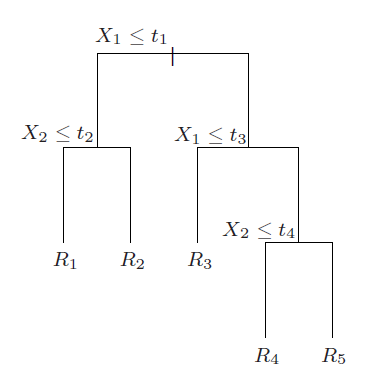
\includegraphics[width=0.25\textwidth]{Documentos Extra/Imagenes/Diagrama de arbol.png}}
 \caption{Representación de la división de $\mathbb{R}^p$ y el diagrama de árbol \\resultante.}
 \label{f:MARC1}
\end{figure}
\end{center}
\end{column}
\end{columns}
\end{frame}
\subsubsection{Árboles de regresión}
\begin{frame}{Métodos supervisados}
\begin{columns}
\begin{column}{0.9\textwidth}
\textbf{Árboles de regresión}

Sea el caso en el que la variable respuesta es cuantitiva y las variables predictoras son cuantitativas o cualitativas.

Tras haber ajustado el árbol hasta tener un tamaño $|T|=M$ resultando en las regiones $R_1,\ldots, R_M$. Entonces el predictor será el siguiente: 
\begin{equation}
\hat{f}(\mathbf{x})=\sum_{m=1}^M \hat{f}_m(\mathbf{x})\cdot \mathbf{1}_m(\mathbf{x})
\end{equation}
donde $\mathbf{1}_m(\mathbf{x})$ es la función característica de la región $R_m,\enspace \forall m=1,\ldots, M$.
\end{column}
\end{columns}
\end{frame}

\begin{frame}{Métodos supervisados}
\begin{columns}
\begin{column}{0.9\textwidth}
\textbf{Árboles de regresión}

Si en cada región queremos que $\hat{f}_m$ sea una constante, $\hat{c}_m$. Utilizando el método de los mínimos cuadrados teniendo en cuenta la restricción de que sea constante se obtiene que: 
\begin{equation}
\hat{c}_m=\dfrac{1}{N_m}\sum_{i/\mathbf{x}_i\in R_m} y_i
\end{equation}
donde $N_m$ es la cantidad de observaciones que hay en la región $R_m \enspace \forall m=1,\ldots M$
\end{column}
\end{columns}
\end{frame}

\begin{frame}{Métodos supervisados}
\begin{columns}
\begin{column}{0.9\textwidth}
\textbf{Árboles de Regresión}

Una partición $(j,s)$ que particione el espacio en las dos regiones $R_{m_1},R_{m_2}$ es elegida si minimiza la siguiente cantidad:
\begin{equation}
\sum_{i/\mathbf{x}_i\in R_{m_1} } (y_i-\hat{c}_{m_1})^2+\sum_{i/\mathbf{x}_i\in R_{m_2} } (y_i-\hat{c}_{m_2})^2
\end{equation}

\end{column}
\end{columns}
\end{frame}
